\usetikzlibrary{decorations}
\usetikzlibrary{snakes}

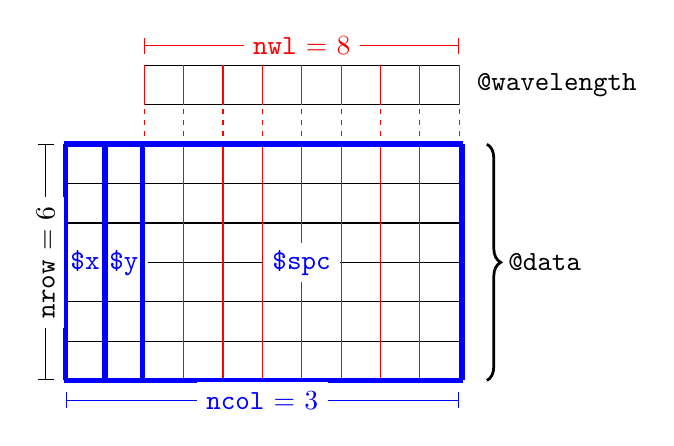
\begin{tikzpicture}[scale=0.5] %Schriftgröße bleibt,
%\draw[fill=red] (0,0) circle (.5);
%\draw[fill=orange] (2,6) circle (.5);
\usetikzlibrary{decorations}
\usetikzlibrary{snakes}

\foreach \x in {0,1,...,10}
 	\foreach \y in {0,1,...,6}
 	\draw (\x,\y) rectangle (1,1);

\foreach \x in {2,3,...,9} \draw (\x,7) rectangle +(1,1);

\draw (0.5,3) node [blue, fill=white,text height=1.5ex,text depth=.25ex] {\texttt{\$x}};
\draw (1.48,3) node [blue, fill=white,text height=1.5ex,text depth=.25ex,] {\texttt{\$y}};

\foreach \x in {2,3,...,10} {
	\draw[color=red] (\x,0) -- (\x,6);
	\draw[color=red, dash pattern=on 2pt off 2pt] (\x,6.9) -- (\x,6.1);
	\draw[color=red] (\x,7) -- (\x,8);
	}

\draw (6,3) node [blue, fill=white,text height=1.5ex,text depth=.25ex] {\texttt{\$spc}};


\foreach \x in {0,1,1.95,10.07} {
	\draw[color=blue, line width=2pt] (\x,0) -- (\x,6);
	}

\foreach \y in {0,6} {
	\draw[line width=2pt, color=blue] (-0.050,\y) -- (10.1,\y);
	}


\draw [<->, >=|, color=red] (2,8.5) -- +(8,0) node [fill=white, pos = 0.5] {\texttt{nwl} = 8};
\draw [<->, >=|, color=blue] (0,-.5) -- +(10,0) node [fill=white, pos = 0.5] {\texttt{ncol} = 3};
\draw [<->, >=|] (-.5,0) -- +(0,6) node [fill=white, pos = 0.5, rotate=90] {\texttt{nrow} = 6};


\draw [snake=brace, segment amplitude=5, mirror snake, raise snake=10, line width=1pt] (10,0) -- (10,6);

\draw (11,3) node [right, ] () {\texttt{@data}};
\draw (10.2,7.5) node [right, ] () {\texttt{@wavelength}};
%\draw (0,0) rectangle ;


\end{tikzpicture}
